\documentclass{article}
\usepackage{tikz}
\usepackage[a3paper, landscape, margin=1in]{geometry}
\usepackage{xcolor}
\usepackage{tikz-qtree}
\usetikzlibrary{arrows,shapes,positioning,shadows,trees}

\tikzset{
  edge from parent fork down,
  sibling distance=60mm,
  all/.style  = {align=center},
  basic/.style  = {all, draw, font=\sffamily, rectangle, sibling distance=20},
  cpp17/.style   = {basic, thin, align=center, fill=lightgray},
  new/.style = {basic, thin,align=center, fill=green!60},
  modified/.style = {basic, thin,align=center, fill=teal!60},
  same/.style = {basic, thin, align=left},
  cppclass/.style = {all, thin, font=\ttfamily}
}

\begin{document}
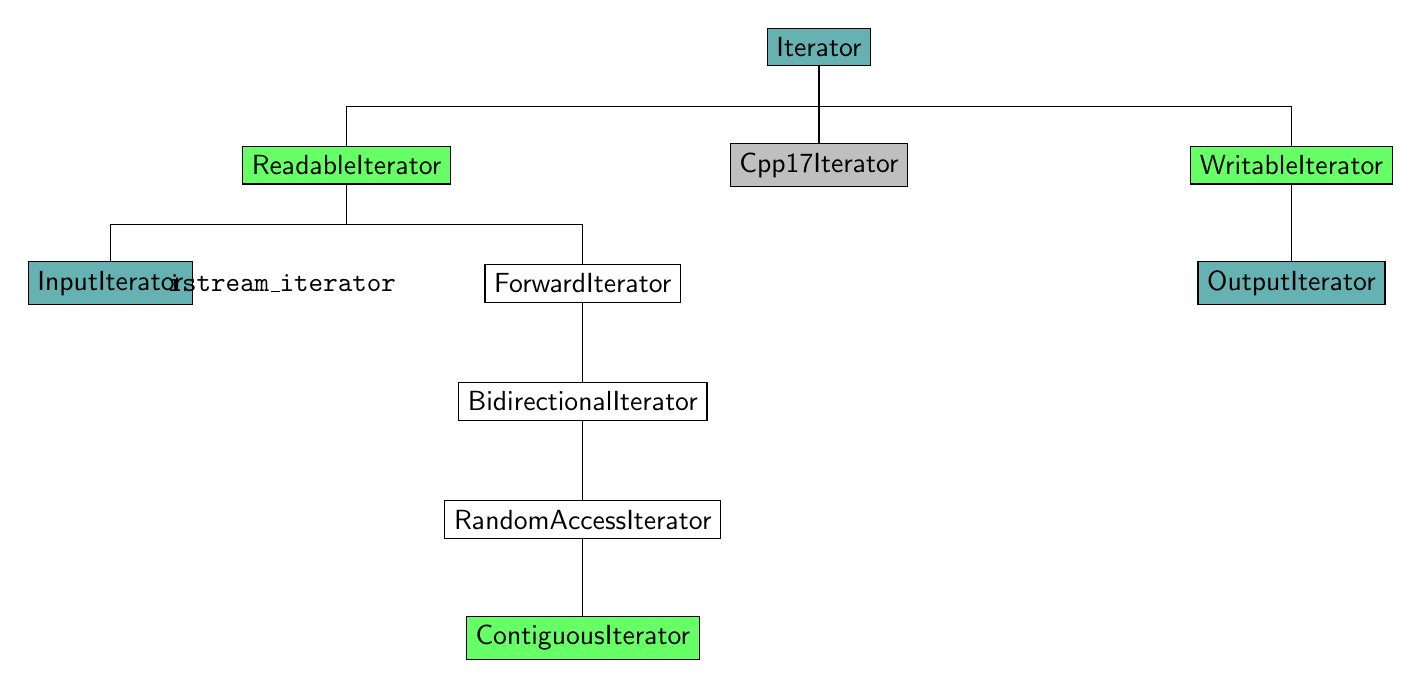
\begin{tikzpicture}
% root of the the initial tree, level 1
\node[modified] {Iterator}
% The first level, as children of the initial tree
  child {node[new] (c1) {ReadableIterator}
  	child {node[modified](InputIterator) {InputIterator}}
  		child {node[same] (FordwardIterator) {ForwardIterator}
  			child {node[same] {BidirectionalIterator}
  				child {node[same] {RandomAccessIterator}
  					child {node[new] {ContiguousIterator}}
  				}
  			}
  		}
  }
  child {node[cpp17] (Cpp17Iterator) {Cpp17Iterator}
  }
  child {node[new] (c3) {WritableIterator}
  	child {node[modified] {OutputIterator}}
  };
  
\node [cppclass,left=of FordwardIterator] (istream) {istream\_iterator};
  
%% \draw[->] (Cpp17Iterator.west) -|  (Cpp17InputIterator.north);
%% \draw[->] (Cpp17Iterator.east) -|  (Cpp17OutputIterator.north);
%% \draw[->] (Cpp17InputIterator.west) -|  (istream.north);

\end{tikzpicture}
\end{document}
